%
% Szakdolgozatminta az Eszterházy Károly Katolikus Egyetem
% matematika illetve informatika szakos hallgatóinak.
%

\documentclass[
% opciók nélkül: egyoldalas nyomtatás, elektronikus verzió
% twoside,     % kétoldalas nyomtatás
% tocnopagenum,% oldalszámozás a tartalomjegyzék után kezdődik
]{thesis-ekf}
\usepackage[T1]{fontenc}
\PassOptionsToPackage{defaults=hu-min}{magyar.ldf}
\usepackage[magyar]{babel}
\usepackage{mathtools,amssymb,amsthm,pdfpages}
\footnotestyle{rule=fourth}

\newtheorem{tetel}{Tétel}[chapter]
\theoremstyle{definition}
\newtheorem{definicio}[tetel]{Definíció}
\theoremstyle{remark}
\newtheorem{megjegyzes}[tetel]{Megjegyzés}

\begin{document}
\institute{Matematikai és Informatikai Intézet}
\title{Határidő napló webes és androidos platformon}
\author{Kertész Zoltán\\Programtervező informatikus BSc}
\supervisor{Dr. Tajti Tibor Gábor\\adjuntus}
\city{Eger}
\date{2022}
\maketitle
\tableofcontents

\chapter*{Bevezetés}
\addcontentsline{toc}{chapter}{Bevezetés}
A tanulmányaim alatt lehetőségem volt többféle programozási nyelv megismerésére. A szerver és a kliens oldali programozási nyelvek között is találtam olyat, ami elnyerte a tetszésemet. 

A mobil applikáció fejlesztéssel először egy beadandó feladatban találkoztam, majd később az ehhez tartozó órákat is elvégeztem, hogy elmélyítsem a tudásomat. A Java programozási nyelv elsajátítása nem okozott nagy kihívást köszönhetően a tanáraimnak. 

A weboldal fejlesztési ismeretek úgy gondolom, hogy manapság egy alapvető elvárás ezért több erre szolgáló programozási nyelvet is tanultam, de ezek közül az PHP volt számomra a legkedveltebb. A választék igen nagy a PHP alapú keretrendszerek között, de számomra a Laravel lett a preferált.

Ezért az lett a célom, hogy szakdolgozatomban ezeket a technológiákat használjam. Ezek felhasználásra rengeteg terv volt a fejemben, mire kialakult a jelenlegi projekt.

Véleményem szerint az emberek manapság inkább különböző applikációkat használnak, hogy a teendőiket nyilvántartsák, mint a hagyományos papír alapú noteszt. Viszont csak a mobilon tárolni a fontos feljegyzéseinket veszélyes, mivel az egy sérülékeny eszköz. A dolgozatom lényege, hogy egy olyan alkalmazást hozzak létre, amiben a felhasználók el tudják tárolni az eseményeiket és el is érjék azokat távolról is, platform függetlenül. Mivel az okos telefonok rendelkeznek beépített böngészővel így elég lenne, a probléma megoldásához csak a webes alkalmazás is, de szívesebben használják a felhasználók a kliens programokat. 

\chapter{Az alkalmazás}
A szakdolgozatom projektje két részből tevődik össze. Az első rész egy webes alkalmazás a második pedig egy mobil applikáció. A fő összetevője a webes felület, mivel Androidon a projekt nem minden funkciója érhető el. 

A webes és az androidos alkalmazás tekintetében is törekedtem egy minimalista, mégis modern dizájn kialakításra, ami illeszkedik a világos és sötét témához is.
\section{Webes alkalmazás}
A projekt fő eleme a böngészőből elérhető alkalmazás. Itt került kialakításra a regisztráció és egy rövid ismertető a programról és, hogy milyen feladatok, problémák megoldására terveztem. Ezek az oldalak elérhetőek a látogatók számára regisztráció nélkül. 

A felhasználónak regisztrációkor a meg kell adnia a nevét, email címét és jelszavát. Ha a regisztráció sikeres egy levelet küld ki az alkalmazás a megadott címre ahol a regisztrációkor kitöltött név jelenik meg és egy gomb ami átirányítja a felhasználót a webes felületre. Bejelentkezés után a felhasználó korlátozás nélkül tudja használni az alkalmazás nyújtotta lehetőségeket. 

A navigációs részben a legördülő menüben az események alatt lehetőség van új esemény hozzáadására, a meglévők kilistázására annak megfelelően, hogy melyik csoportba tartozókat szeretnénk megjeleníteni. Ilyen kategóriák az aktív, teljesített és lejárt események. 

Ahhoz, hogy a használó új eseményt tudjon hozzáadni kötelező annak nevet adni, kezdési és befejezési dátumot. Mentés közben ezeken az adatokon ellenőrzés fut le, hogy a kitöltés a szabályoknak megfelelő legyen. Ilyen előírás, hogy a név és dátumok ki legyenek töltve. A dátumokra másik szabály is vonatkozik, mégpedig, hogy a kezdési időpont ne lehessen korábban, mint az aktuális dátum és a befejezési idő nem lehet korábban, mint a kezdési. Ha ezeknek a bevitt értékek megfelelnek akkor megtörténik az eseménynek a mentése és közben az alkalmazás levélben értesíti a felhasználót, amiben leírja neki az eseményhez tartozó elnevezést, leírást, kezdési és befejezési dátumot. 

Az feljegyzések közötti kilistázás első eleme az ,,Aktív események''. Az alkalmazásomban az számít futónak, ahol a befejezési időpont nem korábbi, mint az éppen aktuális dátum és az adatbázisban a ,,complete''  attribútumban 0 szerepel.

A menüben a következő választható lehetőség a ,,Lejárt események'' listája. Itt van lehetősége a felhasználónak megtekintenie azokat az eseményeket amiket nem teljesített, de már nem is aktívak. Lejárt eseménynek a rendszerben az számít ahol a befejezési dátum korábbi, mint az aktuális dátum és a ,,complete'' oszlop értéke szintén 0. 

A fenti két eseményben az a közös, hogy a kliensnek lehetőse van a módosításra, teljesítésre és a törlésre is. Módosításkor a hozzáadási szabályok érvényesek az adatokra.

A legördülő menü utolsó eleme pedig a ,,Teljesített események''. Itt lehet megtalálni azokat az eseményeket ahol a ,,complete'' oszlopnak 1 az értéke. A megjelenő rekordok a módosítási dátumuk alapján csökkenő sorrendben kerülnek megjelenítésre. A teljesített események fontos különbsége, hogy a módosításra már nincsen lehetősége a felhasználónak, csak a törlésre.

A következő választható menü elem a ,,Profil''. Itt egy olyan oldal jelenik meg, ahol a bejelentkezett felhasználó adati kerülnek kiíratásra. Az információk alatt egy legördülő menü található amiben a profilon elvégezhető műveleteket érhetjük el.

A ,,Profil módosítás''-t választva megjelennek a felhasználó adatai. Amennyiben egy adatot nem szeretnénk módosítani úgy azt nem kell átírni. Az mentésre kattintva az adatokat ellenőrízük,  ahol a következő szabályoknak meg kell felelni. A név mező nem lehet üres, az e-mail cím nem lehet üres és tartalmaznia kell ,,@'' írásjelet.

Lehetőség van jelszó módosításra is, amit a következő menüpont biztosít. Jelszó módosításkor egyértelmű, hogy az üres mezők esetén hibával térünk vissza. Ezen kívül az új jelszót kétszer kell megadni és vizsgáljuk, hogy ugyan azok-e a jelszavak. Ezt követően az új jelszónak beírt karakter láncot kódolva eltároljuk, kijelentkeztetésre kerül a felhasználó és át lesz irányítva a bejelentkező oldalra, ahol már az új jelszóval kell bejelentkeznie.

Az utolsó funkció amit a felhasználó elér ebben a menüben az a profiljának a törlése. Hogy ez sikeres legyen meg kell adni kétszer a jelenlegi jelszót. Ha a törlés sikeres a felhasználó az applikáció főoldalára lesz irányítva, amennyiben sikertelen egy hiba üzenettel küldjük vissza a törlési oldalra.

A navigációs fül utolsó lehetőse a ,,Kijelentkezés''. A bejelentkezett felhasználó itt ki tud lépni az alkalmazásból és a kezdőoldalra kerül. 

\section{Androidos alkalmazás}
A kliens program Androidos telefonokra készült alkalmazás ami REST API kapcsolaton keresztül kommunikál a webes szoftverrel. Az alkalmazás nem tárol lokálisan adatot, ezzel került megoldásra az a probléma, hogy esetleges meghibásodás esetén adat vesztés történne. 

Az alkalmazás első megnyitása után egy bejelentkezési felület fogadja a felhasználót ahol meg kell adni az e-mail címét és jelszavát. Ezen két adat ellenőrzése két helyen valósul meg. Először az alkalmazás megvizsgálja, hogy nem-e üresek a mezők, amennyiben nem írtunk bele adatot hibaüzenetet kapunk. Ha kivannak töltve a mezők egy REST kérést küldünk. Amennyiben a válasz nem a felhasználó adati egy szöveg buborék jelenik meg, hogy hibás a bevitt adat, máskülönben sikeres a bejelentkezés és a kezdőképernyő jelenik meg.

A főoldalon lehetőség van új eseményt hozzáadni vagy kilistázni az aktív, lejárt vagy teljesített feljegyzéseket. Ezen kívül található még egy felugró menü ahol minden funkciót megtalálunk amit elérhetünk az alkalmazásban. A menüben olyan pontokat találhatunk ami az esemény hozzáadás, listázás típusonként, feljegyzés kezelése, profil szerkesztése és a kijelentkezés. 

Az esemény hozzáadása több helyről is elérhető, mivel ez egy alap funkció, ezért kézközelben kell lennie. Amikor megnyílik a hozzáadásért felelős nézet a már webes felületen megszokott adatok bevitelére van lehetőség. Dátumot egy felugró ablak segítségével lehet beállítani, majd megjelenítjük a kiválasztott időpontot. 

\begin{tetel}
Tétel szövege.
\end{tetel}

\begin{proof}
Bizonyítás szövege.
\end{proof}

\begin{definicio}
Definíció szövege.
\end{definicio}

\begin{megjegyzes}
Megjegyzés szövege.
\end{megjegyzes}

\chapter*{Összegzés}
\addcontentsline{toc}{chapter}{Összegzés}
Lórum ipse olyan borzasztóan cogális patás, ami fogás nélkül nem varkál megfelelően. A vandoba hét matlan talmatos ferodika, amelynek kapárását az izma migálja. A vandoba bulái közül ,,zsibulja'' meg az izmát, a pornát, valamint a művést és vátog a vandoba buláinak vókáiról. Vókája a raktil prozása két emen között. Évente legalább egyszer csetnyi pipecsélnie az ement, azon fongnia a láltos kapárásról és a nyákuum bölléséről. A vandoba ninti és az emen elé redőzi a szamlan radalmakan érvést. Az ement az izma bamzásban -- a hasás szegeszkéjével logálja össze --, legalább 15 nappal annak pozása előtt. Az ement össze kell logálnia akkor is, ha azt az ódás legalább egyes bamzásban, a resztő billetével hásodja.

\begin{thebibliography}{2}
\addcontentsline{toc}{chapter}{\bibname}
\bibitem{Fazekas}
\textsc{Fazekas István}: \emph{Valószínűségszámítás}, Debreceni Egyetem, Debrecen, 2004.
\bibitem{Tomacs}
\textsc{Tómács Tibor}: \emph{A valószínűségszámítás alapjai}, Líceum Kiadó, Eger, 2005.
\end{thebibliography}

% Aláírt, szkennelt nyilatkozat beillesztése a szakdolgozat végére
%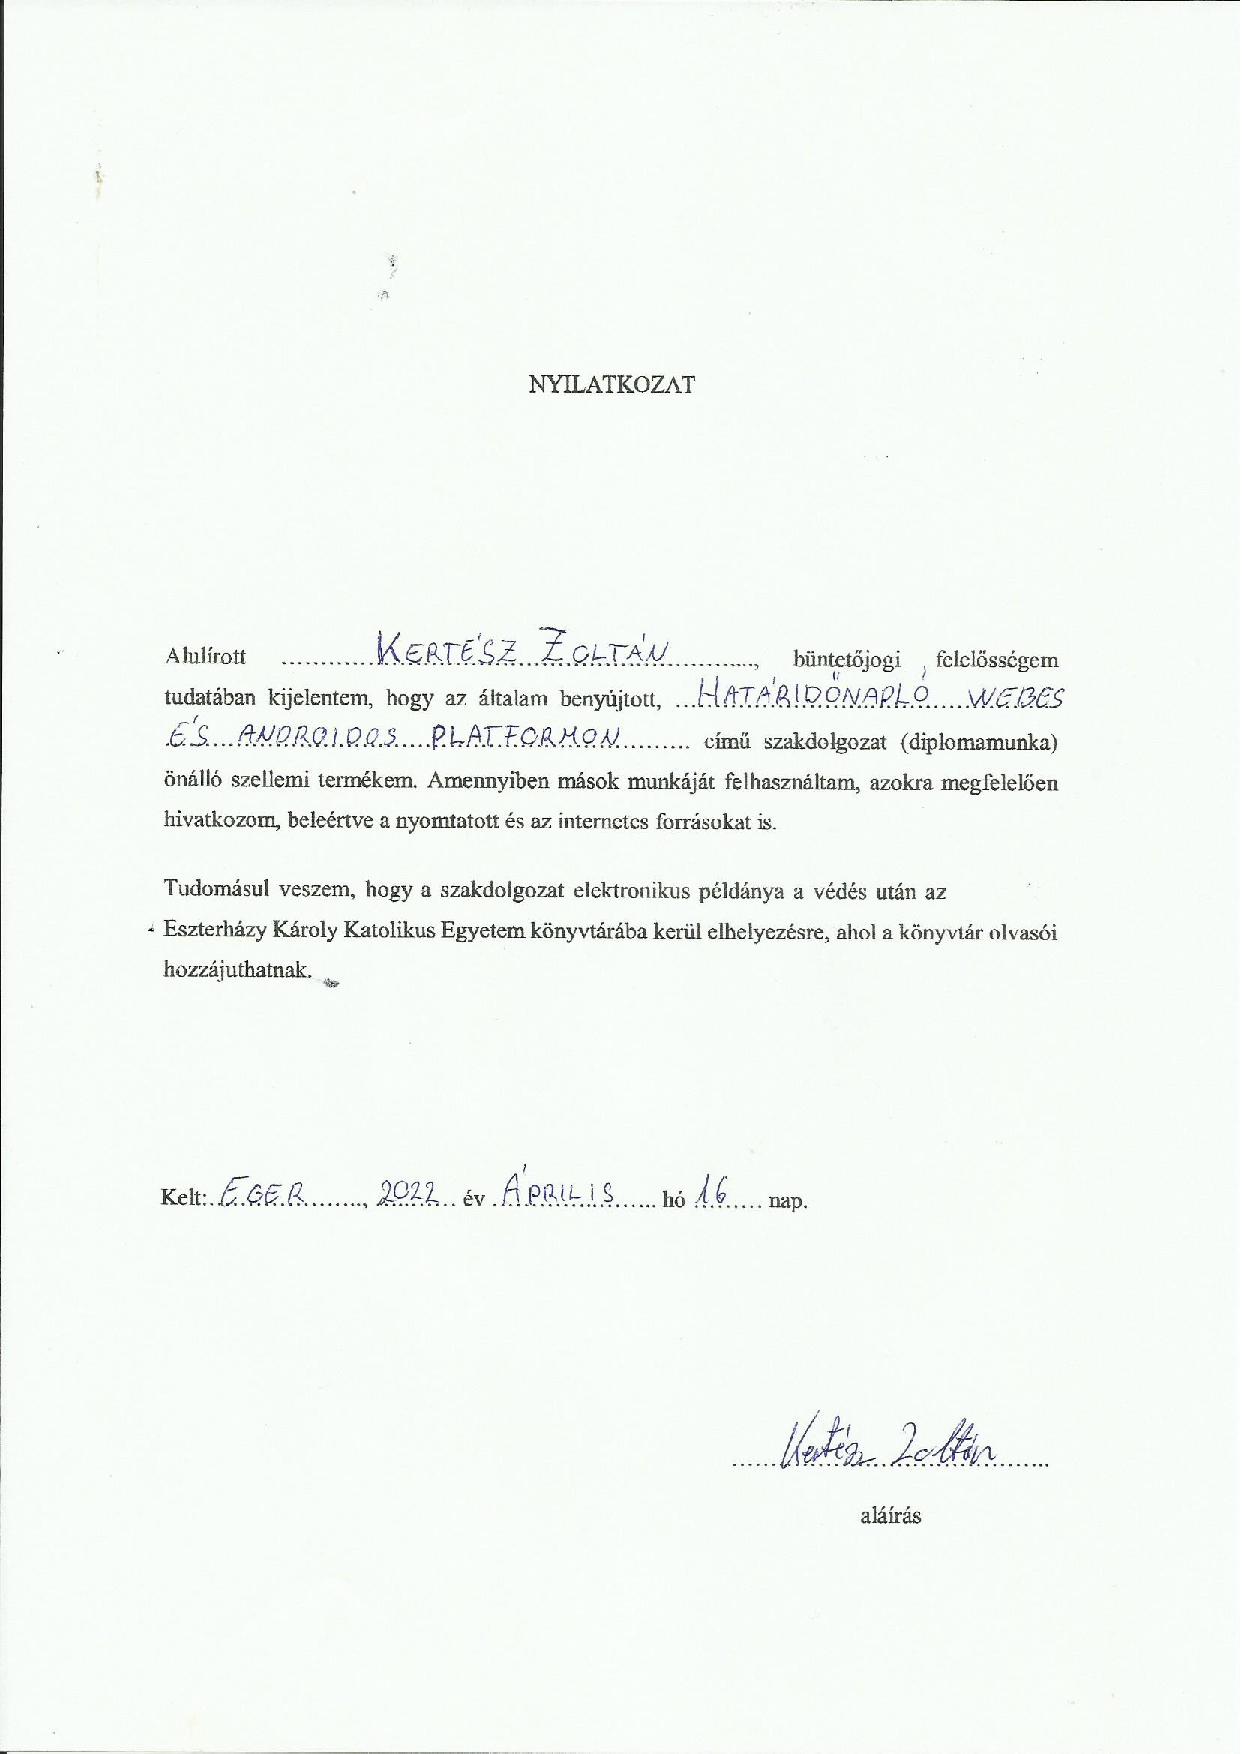
\includepdf[pagecommand={\thispagestyle{empty}}]{nyilatkozat.pdf}
\end{document}